\apendice{Especificación de diseño}

\section{Introducción}
En esta sección se habla sobre la fase de desarrollo software en la que definen la arquitectura, los procedimientos o los datos que se utilizan. Por lo tanto, se da solución

\section{Diseño de datos}

\subsection{Gramática}
Lo referente a la gramática me baso en el trabajo realizado en las anteriores versiones de Thoth\cite{thothv2} y obtengo la parte del núcleo. Según el diagrama obtenido de la documentación del proyecto, la clase Grammar esta compuesta de \emph{Production} y esta a su vez de Symbol. Por medio de la interfaz \emph{TypeHandler} se definen los tipos de gramáticas que existen\ref{fig:4.1}.

\begin{figure}[h]
\centering
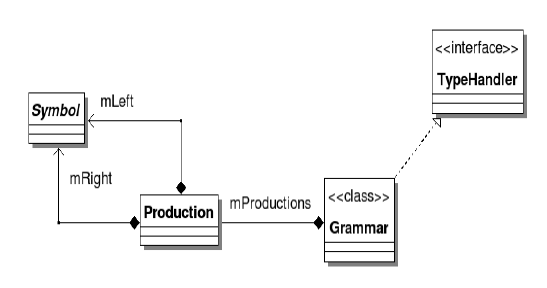
\includegraphics[width=0.50\textwidth]{diseno-gramatica}
\caption{Diagrama de clases del núcleo de la gramática\cite{thothv2}.}
\label{fig:4.1}
\end{figure}


\subsection{Símbolos}

Los símbolos son la unidad mínima con la que se trabajará en una gramática. Los símbolos en una gramática pueden ser terminales, no terminales. La clase NonTerminal estará formada por una cadena de terminales y la clase Terminal trabajará con un único carácter. También se definen los caracteres especiales como son epsilon, o el fin de cadena (TerminalEnd)\ref{fig:4.2}.

\begin{figure}[h]
\centering
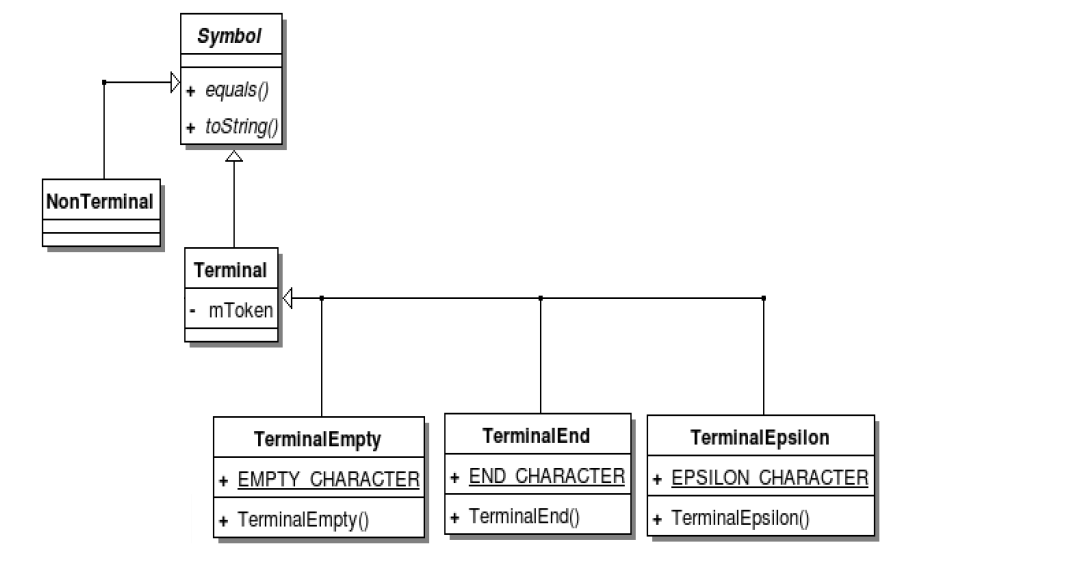
\includegraphics[width=0.60\textwidth]{diseno-simbolo}
\caption{Diagrama de clases de la estructura de Símbolo.}
\label{fig:4.2}
\end{figure}

La especificación de los caracteres que pertenecen a cada tipo viene impuesta por la sintaxis utilizada. Se decidió utilizar minúsculas, dígitos y los operadores básicos ($\ast,+,-,\cdot$) para los terminales. Para los no terminales se determinó que la primera letra debía ir en mayúscula y a ésta le podía seguir cualquier otro terminal o no terminal.

\subsection{Algoritmos de la gramática}

Por simplificación se decide juntar todos los algoritmos de limpieza de gramáticas en un mismo caso dentro del diagrama. Además su estructura es similar entre ellos.

En la figura\ref{fig:4.3} se aprecia como ~los algoritmos de limpieza tienen dos atributos principales, uno correspondiente a la gramática que se desea limpiar, definida como <<mOldGrammar>> y otro que representara la gramática resultante, <<mNewGrammar>>.

\begin{figure}[h]
\centering
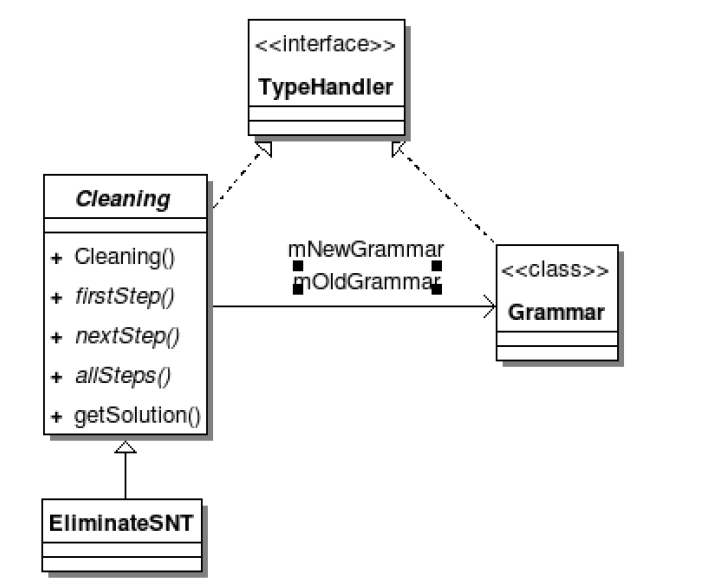
\includegraphics[width=0.40\textwidth]{diseno-algoritmos}
\caption{Diagrama de clases de los Algoritmos de la gramática\cite{thothv2}.}
\label{fig:4.3}
\end{figure}

\subsection{Parser de la gramática}

Aquí se define el diagrama mediante el cual el \emph{parser} analiza la construcción de una gramática, en caso de estar correctamente construida nos crea la estructura interna propia, en caso de contener algún fallo nos muestra un error con el primer símbolo incorrecto encontrado.
A diferencia del parser de expresión regular aquí no se crea ningún árbol de
derivación, en su lugar se va analizando texto plano para ir creando la estructura interna propia.
Esta forma de construcción de gramáticas se ha realizado con el fin de no tener que construir una gramática cada nueva producción, solo se creará la gramática cuando queramos utilizarla (instanciación bajo demanda).

\begin{figure}[h]
\centering
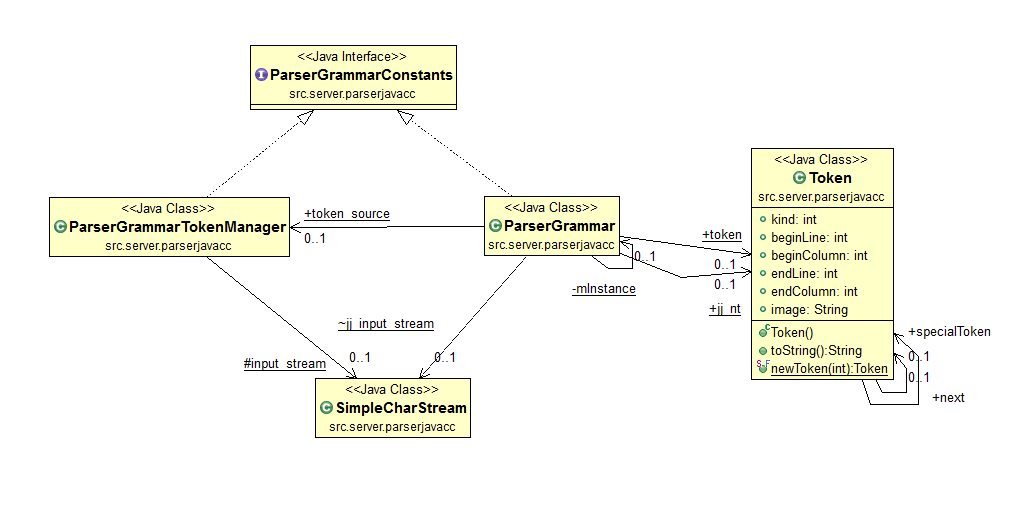
\includegraphics[width=1\textwidth]{diseno-parser}
\caption{Diagrama de clases del Parser de la gramática\cite{thothv2}.}
\label{fig:4.4}
\end{figure}



\subsection{Base de datos}

Este es el diseño de la base de datos para gestionar las sesiones y los registros de usuarios. La clase Login hace de nexo de unión entre las dos vistas, la de registro y la de inicio de sesión. Esa misma clase realiza las peticiones al servidor por medio de las interfaces <<Registration>>. Las interfaces hacen peticiones al \emph{servlet} de registro, <<RegServlet>>, que realizará las operaciones debidas con las base de datos <<dataStoreService>> y con la clase de inicio de sesión <<sessionServlet>> que cargará el módulo que sea según la sesión.

\begin{figure}[h]
\centering
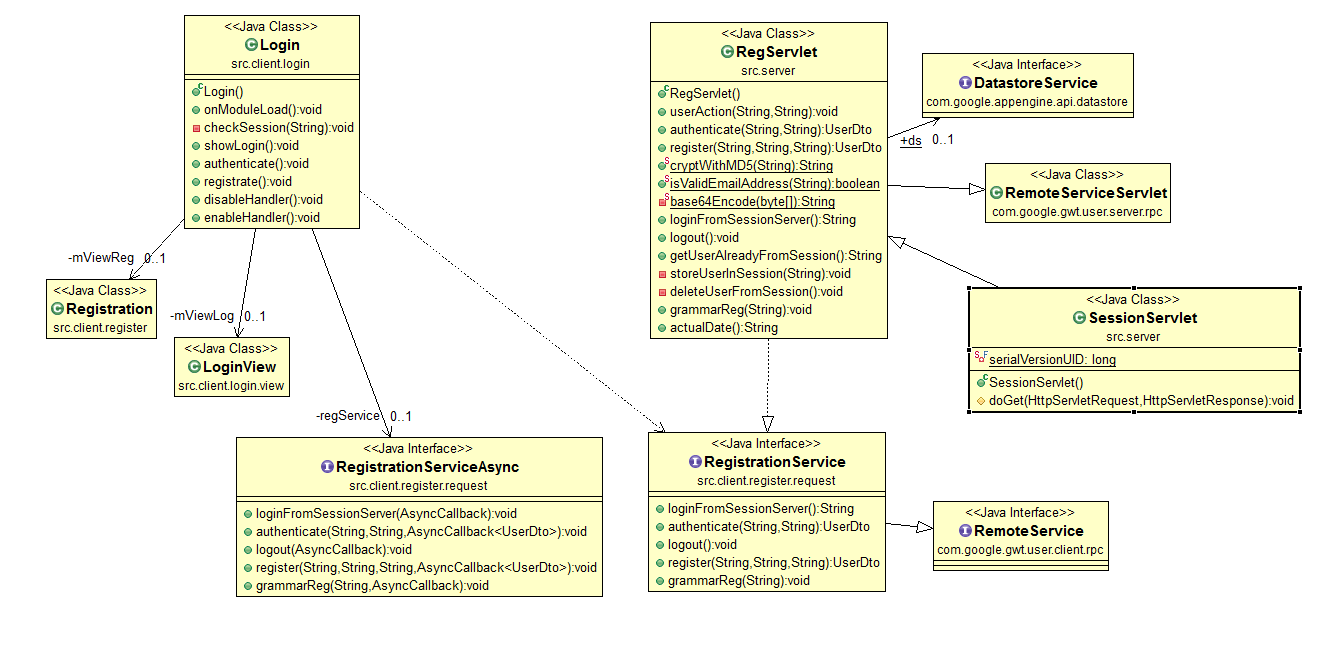
\includegraphics[width=1.1\textwidth]{diseno-inicio-bd}
\caption{Diagrama de clases del Inicio de sesión junto con el registro. Ambos se comunican con la base de datos.}
\label{fig:4.5}
\end{figure}


\section{Diseño procedimental}

Vamos a ver ahora el funcionamiento de varios de los procesos que se llevan a cabo en esta aplicación.
 
Los procesos más importantes en esta aplicación son los dos que se muestran en los siguientes diagramas de flujo. No se representan todos pero si aquellos más importantes que se relacionan con el servidor \ref{fig:4.6}\ref{fig:4.7}.
 \begin{figure}[h]
\centering
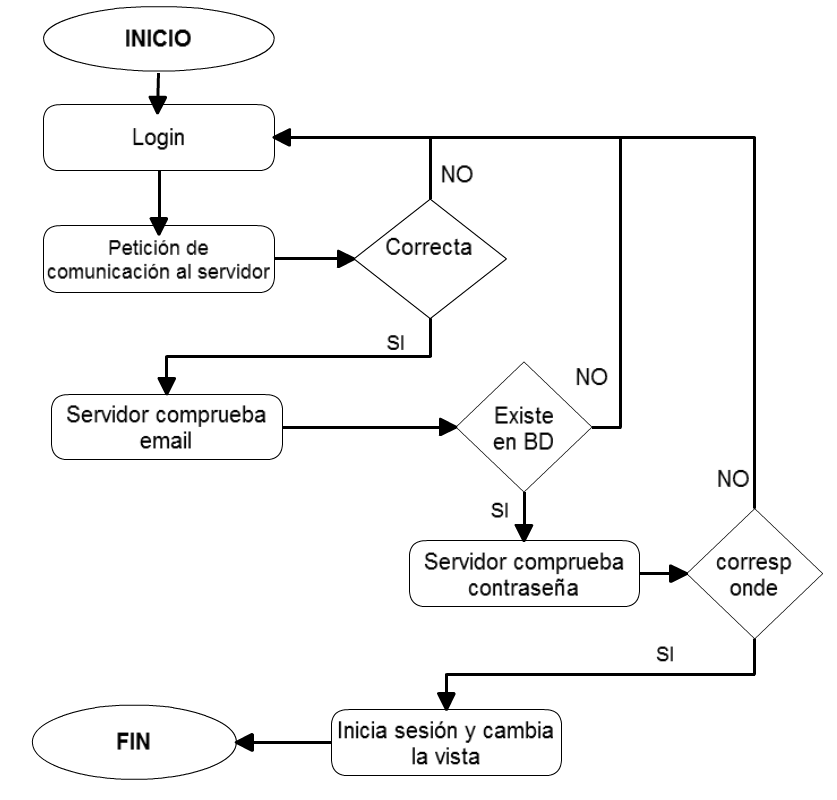
\includegraphics[width=0.80\textwidth]{login-precedimiento}
\caption{Proceso de inicio de sesión en la aplicación.}
\label{fig:4.6}
\end{figure}

\begin{figure}[h]
\centering
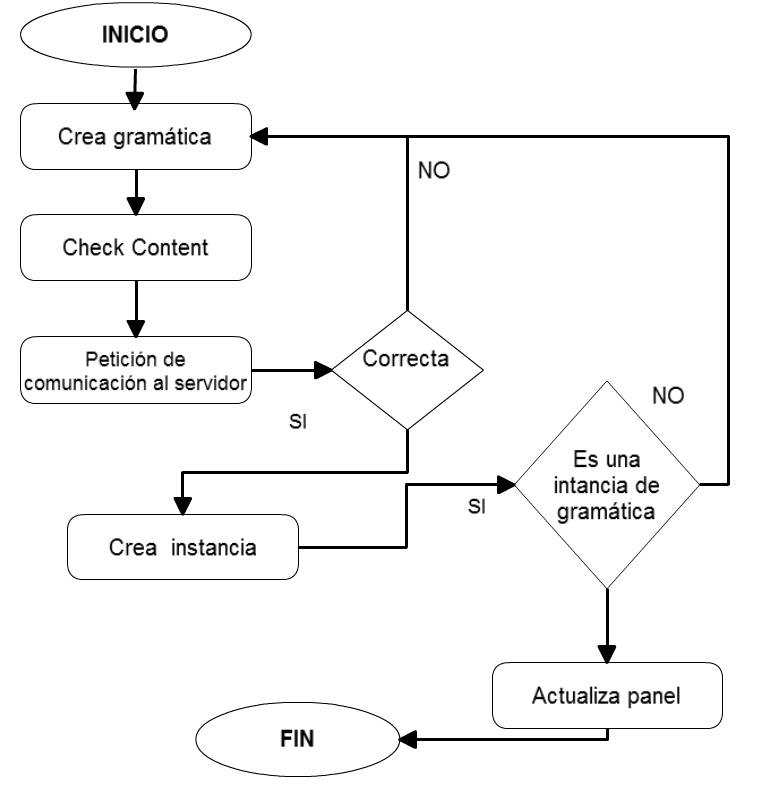
\includegraphics[width=0.80\textwidth]{Comprobar-precedimiento}
\caption{Proceso de comprobación de una gramática.}
\label{fig:4.7}
\end{figure}


\section{Diseño arquitectónico}

En cuanto al diseño arquitectónico, se va a explicar y mostrar de forma general como esta diseñado el proyecto, en cuanto a la distribución de paquetes y los patrones de diseño que se han aplicado.

La aplicación se estructura en tres pilares fundamentales.


\begin{itemize}
\item src:
Este paquete se encuentra todo el código escrito en Java. Esta estructurado en diversas partes siguiendo el diseño modelo-vista-controlador.
	\begin{itemize}
	\item \emph{client}: Aquí se encuentran todos los archivos programados en Java que será traducidos a JavaScript. No pueden contener librerías que no estén especificadas para GWT. Contiene parte del núcleo de Thoth y toda la parte visual de la aplicación.
	\item \emph{server}: En este paquete se guardan las clases que realizan funciones que van a usar librerías no aptas por GWT. Se deben especificar los \emph{servlets} que se utilizan aquí dentro del war. Incluye el parserJavaCC y la base de datos. Su comunicación con el cliente es vía RPC.
	\item \emph{shared}: En este paquete se alojan clases de ayuda entre el cliente y el servidor. Su comunicación es directa, sin RPC, pero tiene las mismas restricciones que el cliente.
	\end{itemize}
\item Test: Contiene las pruebas realizadas sobre diferentes funcionalidades de la aplicación.

\item War:
	Son los archivos que se utilizarán para ejecutar la aplicación en el navegador. Muchos de ellos se generan al compilar la aplicación con GWT. Los html, css y algún xml, están programados por el desarrollador, para configurar la aplicación. GWT genera los archivos con extensión JavaScript, que es la traducción de Java.
\end{itemize}


El proyecto continua con el diseño modelo-vista-controlador de las anteriores versiones de Thoth. 
"Es un patrón de arquitectura de las aplicaciones software. Separa la lógica de negocio de la interfaz de usuario, facilitando la evolución, por separado de ambos aspectos, y aumentando reutilización y flexibilidad" \cite{mvc}.

La estructura de paquetes está definida de la siguiente forma \ref{fig:4.8}. Se puede ver como esta definido el modelo-vista-controlador y como esta agrupados los paquetes según la funcionalidad. Represento solo el cliente porque creo que es el interesante.

\begin{figure}[h]
\centering
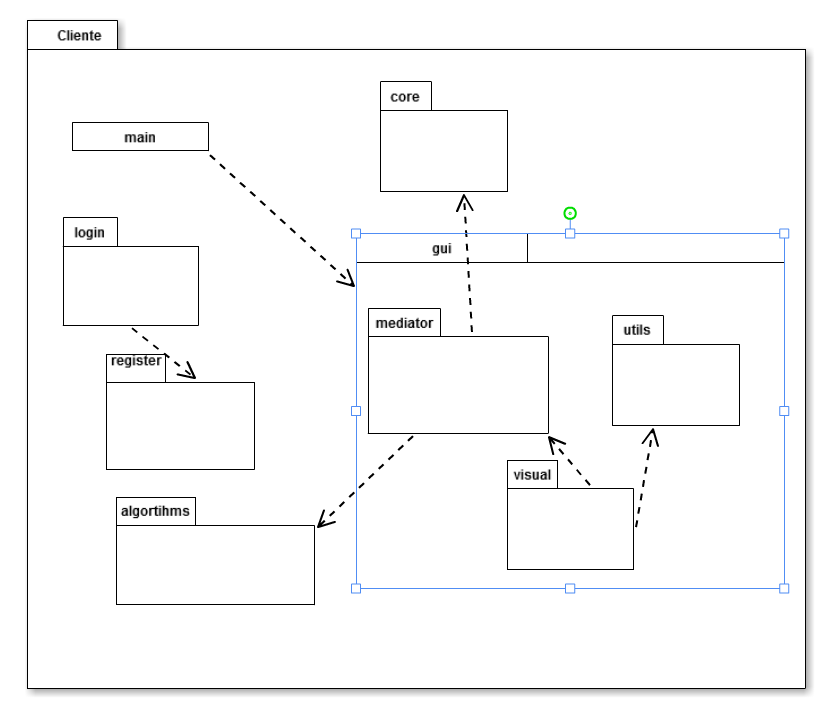
\includegraphics[width=0.80\textwidth]{diagrama-paquetes}
\caption{Diagrama de paquetes dentro de Client.}
\label{fig:4.8}
\end{figure}